\chapter{Tecnologías relacionadas con los componentes}\label{ch:tecnologias-relacionadas-con-los-componentes}

En este capítulo se abordará la creación de un sistema de
vinculación de componentes para \textit{JAMS}, empezando por
la estructura de un componente y terminando por la carga
del mismo dentro de \textit{JAMS}.

También se abordará el desarrollo de las
diferentes tecnologías que permiten a \textit{JAMS}
tener una estructura modular, haciendo que los
componentes puedan alterarla para incluir o modificar
diferentes características.
Cabe destacar que estas tecnologías no solo son usadas
por los componentes, sino que \textbf{el propio \textit{JAMS}}
aprovecha sus virtudes para proporcionar características
dentro del programa principal.

\section{Sistema de vinculación de componentes}\label{sec:sistema-de-vinculacion-de-componentes}

\subsection{Estructura de un componente}\label{subsec:estructura-de-un-componente}

Los componentes, al igual que en muchas aplicaciones \textit{Java},
están conformados por un archivo \textit{jar} con el código que
se desea usar en la aplicación principal.
Más concretamente, un componente de \textit{JAMS} debe contener
dos elementos esenciales:
\begin{itemize}
    \item \textbf{Punto de entrada}: está conformado por una
    clase que extiende a $Plugin$, una clase proporcionada por
    \textit{JAMS} que representa un componente.
    \textit{JAMS} crea una instancia de esta clase para
    poder ejecutar el código externo.
    \item \textbf{Archivo de metadatos}: confirmado por un archivo
    \textit{JSON}\cite{JSON} $plugin.json$ en la raíz del archivo \textit{jar}.
    Este archivo contiene los parámetros globales del componente,
    como pueden ser el \textbf{nombre}, la dirección del
    \textbf{punto de entrada}, la versión, los autores,
    o la descripción.
    Un ejemplo de archivo $plugin.json$ se puede observar en la
    figura \ref{fig:plugin-json}.
\end{itemize}


\begin{figure}[h]
    \centering
    \begin{lstlisting}[frame=single,label={lst:plugin-json}]
{
  "name": "NES4JAMS",
  "main": "io.github.gaeqs.nes4jams.NES4JAMS",
  "version": "0.1-ALPHA",
  "authors": [
    "Gael Rial Costas"
  ],
  "favicon": "/gui/icon/favicon.png",
  "description_node": "NES4JAMS_DESCRIPTION"
}
    \end{lstlisting}
    \caption{Ejemplo de archivo $plugin.json$}
    \label{fig:plugin-json}
\end{figure}

\subsubsection{Dependencias}\label{subsubsec:dependencias}

Un componente puede depender de otro componente.
Para realizar una inicialización correcta de los componentes
se proporcionan los parámetros $dependencies$
y $soft\_dependencies$, los cuales pueden utilizarse en
el archivo $plugin.json$.
Todos los componentes cuyo nombre esté dentro de una de estas
listas serán inicializados con anterioridad.
Si no se encuentra ningún componente que tenga el nombre
de algún valor de $dependencies$, el componente no
se inicializará, lanzando una excepción.
Cabe destacar que dos componentes no pueden conformar
una \textbf{dependencia cíclica}.

\subsubsection{Puntos de entrada}\label{subsubsec:puntos-de-entrada}

Como ya se ha mencionado, un punto de entrada está conformado
por una \textbf{clase que extiende a $Plugin$}.
El desarrollador puede extender dos métodos definidos por esta clase:
$onEnable$ y $onDisable$, que serán llamados cuando el
componente se vincula o desvincula de la aplicación principal.
Un ejemplo de punto de entrada se puede observar en la figura \ref{fig:entry-point}.

\begin{figure}[h]
    \centering
    \begin{lstlisting}[frame=single,label={lst:entry-point},language=Kotlin]
class MyPlugin : Plugin() {

    override fun onEnable() {
        println("My plugin has been enabled!")
        if (JamsApplication.isLoaded()) {
            loadApplicationData()
        }
    }

    override fun onDisable() {
        println("My plugin has been disabled!")
    }

    @Listener
    fun onApplicationLoad(event: JAMSApplicationPostInitEvent)
        = loadApplicationData()

    private fun loadApplicationData() {
        println("Now I can access the JavaFX application!")
    }

}
    \end{lstlisting}
    \caption{Ejemplo de punto de entrada de un componente desarrollado en \textit{Kotlin}}
    \label{fig:entry-point}
\end{figure}

El punto de entrada puede ser inicializado en diferentes
etapas del proyecto: el componente se cargará antes que el contexto
de \textit{JavaFX} si este ya estaba instalado en la aplicación
cuando esta se lanza.
El desarrollador debe \textbf{comprobar si el contexto se ha creado}
antes de añadir o modificar nuevos elementos.
Si el contexto aún no se ha creado, los componentes podrán
usar el evento $JAMSApplicationPostInitEvent$ para ejecutar
código cuando este se inicialice.
Este sistema de eventos se analizará en profundidad más adelante en esta memoria.


\subsection{Vinculación de un componente}\label{subsec:vinculacion-de-un-componente}

Es posible vincular un componente de dos maneras diferentes:
cuando el usuario \textbf{instala el componente} desde la aplicación
y cuando \textbf{se inicializa la aplicación principal} y el componente
está ya instalado.
La vinculación de componentes difiere en varios aspectos en estas
dos situaciones: cuando se instala el componente, \textit{JAMS}
comprueba si \textbf{todas sus dependencias fuertes están presentes}.
Si esto no se cumple, el componente no se instala.
Cuando arranca aplicación principal debe vincular
una cantidad no definida de componentes, y por ello tiene que
generar un \textbf{grafo de dependencias} antes de inicializarlos.

\subsection{Desvinculación de un componente}\label{subsec:desvinculacion-de-un-componente}

Un componente se desvincula de la aplicación principal
cuando \textbf{el usuario lo desinstala} desde
la configuración o cuando la \textbf{aplicación principal se cierra}.
De la misma manera que en la vinculación, el proceso de
desvinculación \textbf{difiere} en ambas circunstancias.
Para que un componente sea desinstalado, el usuario
debe desinstalar previamente \textbf{todos los componentes
que dependen} del componente desinstalado.
Se puede desinstalar el componente cuando no hay
ningún componente dependiente instalado.
Cuando la aplicación principal se cierra
\textbf{no se desvincula ningún componente},
sino que se llama únicamente a sus métodos $onDisable$, dejando
el proceso de desvinculación a la \textit{JVM}.

\subsection{Interfaz de usuario}\label{subsec:interfaz-de-usuario}

Los usuarios pueden instalar o desinstalar componentes
desde la \textbf{ventana de configuración}, mostrada en la figura \ref{fig:plugin-ui}.
En esta interfaz se mostrará la lista de componentes
que están instalados junto con su nombre, su versión
y su descripción.

\begin{figure}[h]
    \centering
    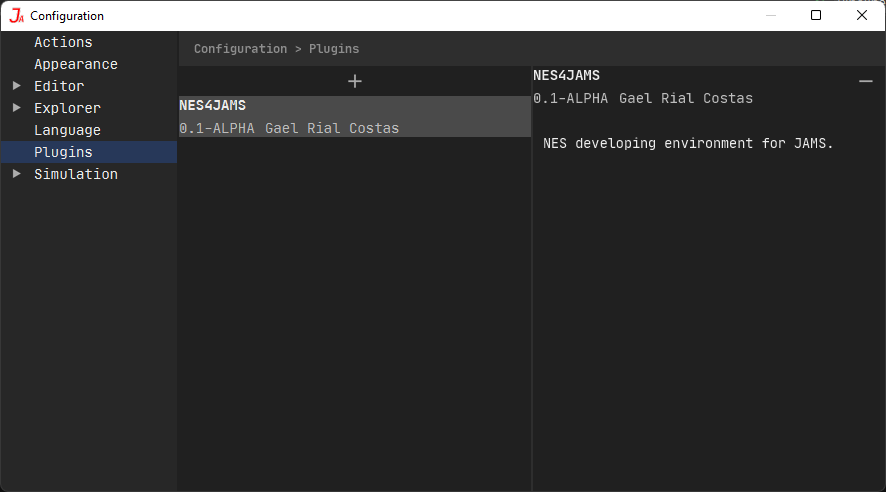
\includegraphics[width=\textwidth]{images/componentes/plugin-ui}
    \caption{Sección de componentes en la configuración}
    \label{fig:plugin-ui}
\end{figure}

\section{Gestores}\label{sec:gestores}

Toda la arquitectura de la aplicación está basada en \textbf{gestores}.
Un gestor se puede definir como un conjunto de elementos que las herramientas pueden utilizar.
\textit{JAMS} proporciona tres tipos básicos de gestores:
\begin{itemize}
    \item \textbf{Gestores normales}: implementados por la clase \textit{Manager}.
    Contienen una lista de elementos sin ninguna jerarquía.
    \item \textbf{Gestores con valor por defecto}: un gestor de este tipo actúa
    como un gestor normal, con la diferencia que uno de sus valores es el valor por defecto.
    Estos gestores heredan de la clase \textit{DefaultValuableManager}.
    \item \textbf{Gestores con valor seleccionado}: actúan como los gestores con valor por defecto,
    pero manteniendo seleccionado uno de los elementos.
    Cuando el elemento seleccionado se elimina, el elemento por
    defecto es el que queda seleccionado en su lugar.
    Estos gestores heredan de la clase \textit{SelectableManager}.
\end{itemize}

\subsection{Proveedores}\label{subsec:proveedores}

Cada elemento guardado en un gestor \textbf{está asociado al proveedor que lo proporciona}.
Un proveedor puede ser un componente o el propio \textit{JAMS}.
Cuando un proveedor se desvincula de la aplicación, todos
los elementos que proporciona son eliminados de los gestores.
Este diseño es una de las principales razones por las que la carga y descarga de
componentes es viable en \textit{JAMS}.
Al tener todos los elementos correctamente etiquetados, \textit{JAMS}
puede retirar los elementos de un componente cuando este se
descarga con una simple llamada a cada gestor.

\subsection{Registro}\label{subsec:registro}

El registro es un \textbf{elemento estático dentro de la aplicación}.
Se le puede considerar como un \textbf{gestor de gestores}.
En el registro se pueden recuperar, añadir, eliminar o modificar gestores.
Igual que sucede con los gestores normales, cuando un proveedor se desvincula de la aplicación,
todos los gestores que proporciona se eliminan del registro.

\textit{JAMS} permite separar los gestores en dos tipos:
\textbf{gestores primarios} y \textbf{gestores secundarios}.
Los gestores primarios son fácilmente accesibles cuando se busca un gestor por tipo
usando métodos como $Manager.of(Type.class)$.
Solo puede existir un gestor primario por tipo.
Para buscar gestores secundarios, se debe proporcionar el nombre del gestor explícitamente.

\subsection{Uso de los gestores}\label{subsec:uso-de-los-gestores}

Como ya se ha indicado, un componente puede añadir, eliminar
y modificar \textbf{los elementos de los gestores y los gestores en sí}.
Definir nuevos gestores es muy sencillo: simplemente se debe crear
una nueva clase que extienda a $Manager$ o a alguno de sus hijos,
como se puede ver en la figura \ref{fig:manager-definition}.

\begin{figure}[h]
    \centering
    \begin{lstlisting}[frame=single,label={lst:manager-definition},language=Kotlin]
data class MyElement(
    private val name: String,
    private val provider: ResourceProvider
) : ManagerResource {
    override fun getName() = name
    override fun getResourceProvider() = provider
}

class MyManager(provider: ResourceProvider) : Manager<MyElement>(
    provider,
    "my-manager",
    MyElement::class.java,
    false
) {
    override fun loadDefaultElements() {}
}
    \end{lstlisting}
    \caption{Definición de un un gestor}
    \label{fig:manager-definition}
\end{figure}

Una vez definido el gestor, este hay que \textbf{registrarlo}.
Para ello, se debe de acceder al registro.
Una vez registrado, cualquier componente podrá acceder al
gestor empleando los métodos proporcionados por el propio \textit{JAMS},
como se observa en la figura \ref{fig:manager-use}.

\begin{figure}[h]
    \centering
    \begin{lstlisting}[frame=single,label={lst:manager-use},language=Kotlin]
class MyPlugin : Plugin() {

    private fun registerAndUseManager() {
        Jams.REGISTRY.registerPrimary(MyManager(this))

        val manager = Manager.of(MyElement::class.java)
        manager.add(MyElement("Test element", this))

        manager.filter { it.name.startsWith("T") }
            .forEach { println(it.name) }
    }
}
    \end{lstlisting}
    \caption{Definición de un un gestor}
    \label{fig:manager-use}
\end{figure}


\section{Eventos}\label{sec:eventos}

\textit{JAMS} incluye un sistema de eventos que permite informar
de sucesos entre componentes de la aplicación.
Este sistema está profundamente inspirado en el sistema de eventos
utilizado por la comunidad de \textit{Minecraft}
en proyectos como \textit{Spigot}\cite{SPIGOT}
o \textit{Sponge}\cite{SPONGE}, y puede considerarse una evolución descentralizada
de esta tecnología.

\subsection{Emisores de eventos}\label{subsec:emisores-de-eventos}

Los emisores de eventos son los encargados de transmitir
eventos a los elementos que los escuchan.
Los diferentes creadores de eventos los transmitirán a través de un
canal que será utilizado también por los elementos que estén
escuchando a la espera de recibirlos.

Un emisor de eventos está representado por la interfaz $EventBroadcast$.
Esta interfaz es implementada por cualquier elemento que pueda emplearse para registrar escuchas.
Los gestores, los componentes o el propio \textit{JAMS} implementan
un emisor por defecto.
La clase $SimpleEventBroadcast$ contiene una implementación de $EventBroadcast$
que puede utilizarse como superclase.

\subsection{Definir escuchas}\label{subsec:definir-escuchas}

Las escuchas son \textbf{métodos no estáticos marcados con la anotación @Listener}.
Estos métodos solo tienen un parámetro que pide un elemento que extienda la clase
$Event$ y deben devolver $void$.
Este método, después de ser registrado en un gestor de idiomas,
se ejecutará cuando se añada un nuevo idioma.
En la figura \ref{fig:listener} se observa una escucha de ejemplo.

\begin{figure}[h]
    \centering
    \begin{lstlisting}[frame=single,label={lst:listener},language=Kotlin]
@Listener
fun onLanguageRegister(
    event: ManagerElementRegisterEvent.After<Language>
) {
    println("New language available! ${event.element.name}")
}
    \end{lstlisting}
    \caption{Objeto registrando un evento en el emisor general de \textit{JAMS}}
    \label{fig:listener}
\end{figure}

A diferencia de otros sistemas similares,
el sistema de eventos de \textit{JAMS} permite usar \textbf{eventos genéricos}.
Un ejemplo es el caso anterior, donde el método solicita un elemento de tipo
$ManagerElementRegisterEvent.After<Language>$.
Si el emisor al que está registrado emite un evento de tipo
$ManagerElementRegisterEvent.After<Theme>$, la escucha no será invocada.

Un evento puede extender la clase de otro evento.
Esto permite generar una jerarquía de eventos.
Una escucha que pide un cierto tipo de evento se ejecutará siempre
que se produzca dicho evento o uno de sus hijos.
Si una escucha \delODR{pide el}\newODR{¿invoca al?} evento $Event$,
su método se ejecutará siempre que ocurra un evento.

Algunos eventos implementan la interfaz $Cancellable$, lo cual permite cancelar el evento.
Las escuchas restantes no serán llamadas cuando se cancela un evento salvo que se defina lo contrario
en la anotación $@Listener$.

\subsection{Registrar escuchas}\label{subsec:registrar-escuchas}

Una vez un objeto tenga definidas todas sus escuchas, estas
pueden registrarse en uno o varios emisores de eventos.
Para ello se debe llamar al método $registerListeners$ del
emisor deseado, tal y como se muestra en la figura \ref{fig:event-registration}.

\begin{figure}[h]
    \centering
    \begin{lstlisting}[frame=single,label={lst:event-registration-use},language=Kotlin]
class ObjectWithListeners {

    init {
        Jams.getGeneralEventBroadcast().registerListeners(
            /* instance = */ this,
            /* useWeakReferences = */ true
        )
    }

    @Listener
    private fun onEvent(event: Event) {
        println("I received a new event! $event")
    }

}
    \end{lstlisting}
    \caption{Objeto registrando un evento en el emisor general de \textit{JAMS}}
    \label{fig:event-registration}
\end{figure}

El método de registro pide dos variables: el objeto
con las escuchas y si se deben emplear \textbf{referencias débiles}.
Esta última opción permite que los objetos sean eliminados de la memoria
cuando ya no resulten necesarios, incluso aunque tengan escuchas registradas.
Estas escuchas \textbf{se eliminarán del emisor automáticamente} si no existe
ninguna referencia al objeto (sin contar la del propio emisor).
Esto permite desarrollar componentes de una manera \textbf{muy sencilla}:
combinado con el sistema de proveedores, las referencias débiles
de las escuchas evitan que la aplicación mantenga elementos de un
componente cuando este se desinstala.

Por último, cabe destacar que el método de registro
busca todos los métodos de escucha de un objeto,
\textbf{ampliando la búsqueda a los métodos de las clases padre}.
Esto permite heredar funcionalidades de objetos ya programados
de manera sencilla.
Si el desarrollador desea registrar un único método puede hacerlo
con los métodos proporcionados, pero para ello se requieren
conocimientos de la librería \textit{reflection} de \textit{Java}.


\section{Tareas}\label{sec:tareas}

Las tareas son elementos muy importantes dentro de una aplicación
de escritorio.
Consisten en \textbf{funciones que ejecutan una tarea de manera
asíncrona al hilo principal} de la aplicación, devolviendo un
resultado al finalizar su ejecución.
\textit{Java} proporciona diversas maneras de gestionar
las tareas dentro de una aplicación, y \textit{JavaFX}
también implementa su propia solución.
Por ello \textit{JAMS} proporciona una pequeña
librería que permite a los desarrolladores ejecutar
tareas \textbf{visibles por el usuario} en la barra
de proceso de la ventana principal de la aplicación.

\textit{JAMS} implementa por defecto un
sistema de tareas basado en \textbf{ejecutor}.
Un ejecutor es un conjunto de hilos que ejecutan
diversas tareas.
Cada proyecto presenta un ejecutor único por defecto,
lo que permite los desarrolladores lanzar tareas de una
manera sencilla, como se puede observar en la figura \ref{fig:tasks-execution}.

\begin{figure}[h]
    \centering
    \begin{lstlisting}[frame=single,label={lst:tasks-execution},language=Kotlin]
fun startTask(project: Project) {
    project.taskExecutor.execute(
        LanguageTask.of("MY_TITLE_LANGUAGE_NODE") {
            Thread.sleep(1000)

            // Do things here!

            Thread.sleep(1000)
    })
}
    \end{lstlisting}
    \caption{Inicialización de una tarea con título}
    \label{fig:tasks-execution}
\end{figure}

Las tareas creadas con la clase $LanguageTask$
pueden tener un título y una descripción que cambian dependiendo
del idioma seleccionado por el usuario.
Ambos son visibles al usuario, y se muestran
en la barra inferior de la ventana principal de \textit{JAMS},
como se puede ver en la figura \ref{fig:jams-assembling}.

\begin{figure}[h]
    \centering
    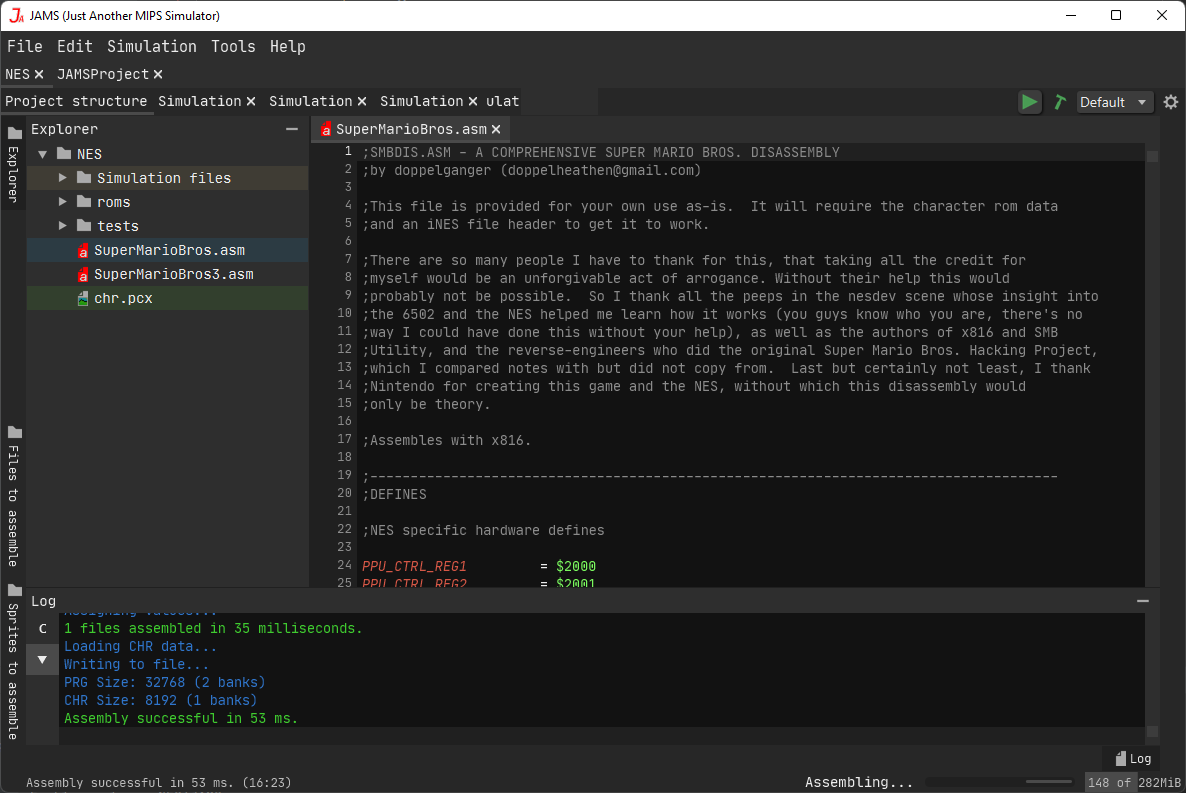
\includegraphics[width=\textwidth]{images/tecnologias/jams-assembling}
    \caption{\textit{JAMS} ejecutando una tarea de ensamblaje}
    \label{fig:jams-assembling}
\end{figure}